\section{Εισαγωγή}
Τα γραφήματα είναι δομές δεδομένων που συναντώνται συχνά κατά την επίλυση προβλημάτων. Η ευχέρεια προγραμματισμού αλγορίθμων που εφαρμόζονται πάνω σε γραφήματα είναι ουσιώδης. Καθώς μάλιστα συχνά ανακύπτουν προβλήματα για τα οποία έχουν διατυπωθεί αλγόριθμοι αποδοτικής επίλυσής τους η γνώση των αλγορίθμων αυτών αποδεικνύεται ισχυρός σύμμαχος στην επίλυση δύσκολων προβλημάτων. 

\section{Γραφήματα}
Ένα γράφημα ή γράφος (graph) είναι ένα σύνολο από σημεία που ονομάζονται κορυφές (vertices) ή κόμβοι (nodes) για τα οποία ισχύει ότι κάποια από αυτά είναι συνδεδεμένα απευθείας μεταξύ τους με τμήματα γραμμών που ονομάζονται ακμές (edges ή arcs). Συνήθως ένα γράφημα συμβολίζεται ως $G=(V,E)$ όπου $V$ είναι το σύνολο των κορυφών και $E$ είναι το σύνολο των ακμών.

Αν οι ακμές δεν έχουν κατεύθυνση τότε το γράφημα ονομάζεται μη κατευθυνόμενο (undirected) ενώ σε άλλη περίπτωση ονομάζεται κατευθυνόμενο (directed). Ένα πλήρες γράφημα (που όλες οι κορυφές συνδέονται απευθείας με όλες τις άλλες κορυφές) έχει $\frac{|V||V-1|}{2}$ ακμές ($|V|$ είναι το πλήθος των κορυφών του γραφήματος). Αν σε κάθε ακμή αντιστοιχεί μια τιμή τότε το γράφημα λέγεται γράφημα με βάρη. Το γράφημα του σχήματος \ref{fig:undirected_graph1} είναι ένα μη κατευθυνόμενο γράφημα με βάρη. 

\begin{figure}[ht]
	\centering
	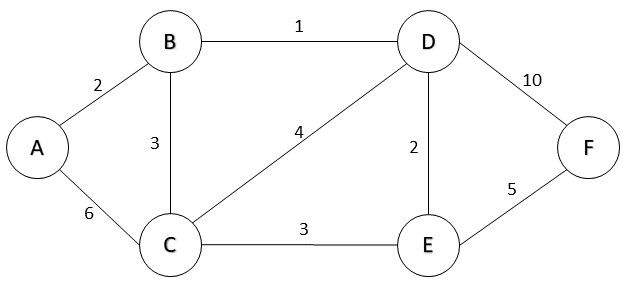
\includegraphics[width=100mm]{undirected_graph1.png}
	\caption{Ένα μη κατευθυνόμενο γράφημα 6 κορυφών και 9 ακμών με βάρη στις ακμές του}
	\label{fig:undirected_graph1}
\end{figure}

Ένα γράφημα λέγεται συνεκτικό αν για δύο οποιεσδήποτε κορυφές του υπάρχει μονοπάτι που τις συνδέει. Αν ένα γράφημα δεν είναι συνεκτικό τότε αποτελείται από επιμέρους συνεκτικά γραφήματα τα οποία λέγονται συνιστώσες. Είναι προφανές ότι ένα συνεκτικό γράφημα έχει μόνο μια συνιστώσα.

\subsection{Αναπαράσταση γραφημάτων}
Δύο διαδεδομένοι τρόποι αναπαράστασης γραφημάτων είναι οι πίνακες γειτνίασης (adjacency matrices) και οι λίστες γειτνίασης (adjacency lists).

Στους πίνακες γειτνίασης διατηρείται ένας δισδιάστατος πίνακας $n \times n$ όπου $n$ είναι το πλήθος των κορυφών του γραφήματος. Για κάθε ακμή του γραφήματος που συνενώνει την κορυφή $i$ με την κορυφή $j$ εισάγεται στη θέση $i,j$ του πίνακα το βάρος της ακμής αν το γράφημα είναι με βάρη ενώ αν δεν υπάρχουν βάρη τότε εισάγεται η τιμή 1. Όλα τα υπόλοιπα στοιχεία του πίνακα λαμβάνουν την τιμή 0. Για παράδειγμα η πληροφορία του γραφήματος για το σχήμα \ref{fig:undirected_graph1} διατηρείται όπως φαίνεται στον πίνακα \ref{tbl:adjacency_table}.

% Please add the following required packages to your document preamble:
% \usepackage[table,xcdraw]{xcolor}
% If you use beamer only pass "xcolor=table" option, i.e. \documentclass[xcolor=table]{beamer}
\begin{table}[ht]
	\centering
	\begin{tabular}{|
		>{\columncolor[HTML]{C0C0C0}}l |c|c|c|c|c|c|}
		\hline
		\cellcolor[HTML]{FFFFFF} & \cellcolor[HTML]{C0C0C0} A & \cellcolor[HTML]{C0C0C0} B & \cellcolor[HTML]{C0C0C0} C & \cellcolor[HTML]{C0C0C0}D & \cellcolor[HTML]{C0C0C0} E & \cellcolor[HTML]{C0C0C0} F \\ \hline
		A                        & 0                          & 2                          & 6                          & 0                         & 0                          & 0                          \\ \hline
		B                        & 2                          & 0                          & 3                          & 1                         & 0                          & 0                          \\ \hline
		C                        & 6                          & 3                          & 0                          & 4                         & 3                          & 0                          \\ \hline
		D                        & 0                          & 1                          & 4                          & 0                         & 2                          & 10                         \\ \hline
		E                        & 0                          & 0                          & 3                          & 2                         & 0                          & 5                          \\ \hline
		F                        & 0                          & 0                          & 0                          & 10                        & 5                          & 0                          \\ \hline
	\end{tabular}
	\caption{Πίνακας γειτνίασης για το σχήμα \ref{fig:undirected_graph1}}
    \label{tbl:adjacency_table}
\end{table}

Στις λίστες γειτνίασης διατηρούνται λίστες που περιέχουν για κάθε κορυφή όλη την πληροφορία των συνδέσεών της με τους γειτονικούς της κόμβους. Για παράδειγμα το γράφημα του σχήματος \ref{fig:undirected_graph1} μπορεί να αναπαρασταθεί με τις ακόλουθες 6 λίστες (μια ανά κορυφή). Κάθε στοιχείο της λίστας για την κορυφή $v$ είναι ένα ζεύγος τιμών $(w,u)$ και αναπαριστά μια ακμή από την κορυφή $v$ στην κορυφή $u$ με βάρος $w$, όπως φαίνεται στο πίνακα \ref{tbl:adjacency_list}.

\begin{table}[ht]
	\centering
	\begin{tabular}{|
		>{\columncolor[HTML]{C0C0C0}}l |c|}
		\hline
		A & (2,B), (6,C)                \\ \hline
		B & (2,A), (3,C), (1,D)         \\ \hline
		C & (6,A), (3,B), (4,D), (3,E)  \\ \hline
		D & (1,B), (4,C), (2,E), (10,F) \\ \hline
		E & (3,C), (2,D), (5,F)         \\ \hline
		F & (10,D), (5,E)               \\ \hline
	\end{tabular}
	\caption{Λίστα γειτνίασης για το σχήμα \ref{fig:undirected_graph1}}
	\label{tbl:adjacency_list}
\end{table}

Περισσότερα για τις αναπαραστάσεις γραφημάτων μπορούν να βρεθούν στις αναφορές \cite{g4g_graph_representations} και \cite{he_graph_representations}.

\subsection{Ανάγνωση δεδομένων γραφήματος από αρχείο}
Υπάρχουν πολλοί τρόποι με τους οποίους μπορούν να βρίσκονται καταγεγραμμένα τα δεδομένα ενός γραφήματος σε ένα αρχείο. Το αρχείο αυτό θα πρέπει να διαβαστεί έτσι ώστε να αναπαρασταθεί το γράφημα στη μνήμη του υπολογιστή. Στη συνέχεια παρουσιάζεται μια απλή μορφή αποτύπωσης κατευθυνόμενων με βάρη γραφημάτων χρησιμοποιώντας αρχεία απλού κειμένου. Σύμφωνα με αυτή τη μορφή για κάθε κορυφή του γραφήματος καταγράφεται σε ξεχωριστή γραμμή του αρχείου κειμένου το όνομά της ακολουθούμενο από ζεύγη τιμών, χωρισμένων με κόμματα, που αντιστοιχούν στις ακμές που ξεκινούν από τη συγκεκριμένη κορυφή. Στο κείμενο που ακολουθεί (graph1.txt) και το οποίο αφορά το γράφημα του σχήματος \ref{fig:undirected_graph1} η πρώτη γραμμή σημαίνει ότι η κορυφή Α συνδέεται με μια ακμή με βάρος 2 με την κορυφή B καθώς και με μια ακμή με βάρος 6 με την κορυφή C. Ανάλογα καταγράφεται η πληροφορία ακμών και για τις άλλες κορυφές.

\lstinputlisting[style=DOS]{lab08/graph1.txt}

Η ανάγνωση του αρχείου και η αναπαράσταση του γραφήματος ως λίστα γειτνίασης γίνεται με τη συνάρτηση read\_data που δίνεται στη συνέχεια όπου fn είναι το όνομα του αρχείου. Η συνάρτηση αυτή δημιουργεί ένα λεξικό (map) που αποτελείται από εγγραφές τύπου key-value. Σε κάθε εγγραφή το key είναι ένα λεκτικό με το όνομα μιας κορυφής ενώ το value είναι ένα διάνυσμα (vector) που περιέχει ζεύγη (pair<int,string>) στα οποία το πρώτο στοιχείο είναι ένας ακέραιος αριθμός που αναπαριστά το βάρος μιας ακμής ενώ το δεύτερο ένα λεκτικό με το όνομα της κορυφής στην οποία καταλήγει η ακμή από την κορυφή key. Ο κώδικας έχει ``σπάσει'' σε 3 αρχεία (graph.hpp, graph.cpp και graph\_ex1.cpp) έτσι ώστε να είναι ευκολότερη η επαναχρησιμοποίηση του. Η συνάρτηση print\_data εμφανίζει τα δεδομένα του γραφήματος.

\lstinputlisting[caption = header file με τις συναρτήσεις για ανάγνωση και εμφάνιση γραφημάτων (graph.hpp)]{lab08/graph.hpp}

\lstinputlisting[caption = source file με τις συναρτήσεις για ανάγνωση και εμφάνιση γραφημάτων (graph.cpp),multicols=2]{lab08/graph.cpp}

\lstinputlisting[caption = Ανάγνωση και εκτύπωση των δεδομένων του γραφήματος του σχήματος \ref{fig:undirected_graph1} (graph\_ex1.cpp)]{lab08/graph_ex1.cpp}

Η μεταγλώττιση και η εκτέλεση του κώδικα γίνεται με τις ακόλουθες εντολές:

\lstinputlisting[style=DOS]{lab08/compile_execute1.txt}

Η δε έξοδος που παράγεται είναι η ακόλουθη:

\lstinputlisting[style=DOS]{lab08/graph_ex1.out}

\subsection{Κατευθυνόμενα ακυκλικά γραφήματα}
Τα κατευθυνόμενα ακυκλικά γραφήματα (Directed Acyclic Graphs=DAGs) είναι γραφήματα για τα οποία δεν μπορεί να εντοπιστεί διαδρομή από μια κορυφή προς την ίδια. Στο σχήμα \ref{fig:dag1} παρουσιάζεται ένα γράφημα το οποίο δεν παρουσιάζει κύκλους. Αν για παράδειγμα υπήρχε μια ακόμα ακμή από την κορυφή E προς την κορυφή A τότε πλέον το γράφημα δεν θα ήταν DAG καθώς θα υπήρχε ο κύκλος A-C-E-A.

\begin{figure}[ht]
	\centering
	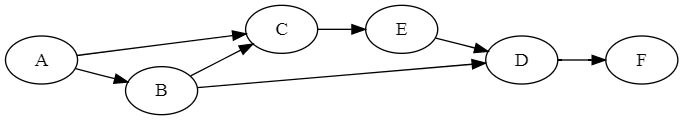
\includegraphics[width=120mm]{dag1.png}
	\caption{Ένα κατευθυνόμενο ακυκλικό γράφημα (DAG)}
	\label{fig:dag1}
\end{figure}

Τα DAGs χρησιμοποιούνται στη μοντελοποίηση πολλών καταστάσεων. Μπορούν για παράδειγμα να αναπαραστήσουν εργασίες που πρέπει να εκτελεστούν και για τις οποίες υπάρχουν εξαρτήσεις όπως για παράδειγμα ότι για να ξεκινήσει η εκτέλεση της εργασίας D θα πρέπει πρώτα να έχουν ολοκληρωθεί οι εργασίες B και E. 

\subsection{Σημαντικοί αλγόριθμοι γραφημάτων}
Υπάρχουν πολλοί αλγόριθμοι που εφαρμόζονται σε γραφήματα προκειμένου να επιλύσουν ενδιαφέροντα προβλήματα που ανακύπτουν σε πρακτικές εφαρμογές. Οι ακόλουθοι αλγόριθμοι είναι μερικοί από αυτούς:
\begin{itemize}[noitemsep]
	\item Αναζήτηση συντομότερων διαδρομών από μια κορυφή προς όλες τις άλλες κορυφές (Dijkstra). Ο αλγόριθμος αυτός θα αναλυθεί στη συνέχεια.
	\item Εύρεση μήκους συντομότερων διαδρομών για όλα τα ζεύγη κορυφών (Floyd Warshall) \cite{pa_floyd_warshall}.
	\item Αναζήτηση κατά βάθος (Depth First Search). Είναι αλγόριθμος διάσχισης γραφήματος ο οποίος ξεκινά από έναν κόμβο αφετηρία και επισκέπτεται όλους τους άλλους κόμβους που είναι προσβάσιμοι χρησιμοποιώντας της ακμές του γραφήματος. Λειτουργεί επεκτείνοντας μια διαδρομή όσο βρίσκει νέους κόμβους τους οποίους μπορεί να επισκεφθεί. Αν δεν βρίσκει νέους κόμβους οπισθοδρομεί και διερευνά άλλα τμήματα του γραφήματος.
	\item Αναζήτηση κατά πλάτος (Breadth First Search). Αλγόριθμος διάσχισης γραφήματος που ξεκινώντας από έναν κόμβο αφετηρία επισκέπτεται τους υπόλοιπους κόμβους σε αύξουσα σειρά βημάτων από την αφετηρία. Βήματα θεωρούνται οι μεταβάσεις από κορυφή σε κορυφή.
	\item Εντοπισμός ελάχιστου συνεκτικού (ή γεννητικού) δένδρου (Prim \cite{programiz_prim}, Kruskal \cite{programiz_kruskal}). Δεδομένου ενός γραφήματος, το πρόβλημα αφορά την εύρεση ενός δένδρου στο οποίο θα περιέχονται όλες οι κορυφές του γραφήματος ενώ οι ακμές του δένδρου θα είναι ένα υποσύνολο των ακμών του γραφήματος τέτοιο ώστε το άθροισμα των βαρών τους να είναι το ελάχιστο δυνατό.
	\item Τοπολογική ταξινόμηση (Topological Sort) \cite{g4g_topological_sort}. Ο αλγόριθμος τοπολογικής ταξινόμησης εφαρμόζεται σε DAGs και παράγει μια σειρά κορυφών του γραφήματος για την οποία ισχύει ότι για κάθε κατευθυνόμενη ακμή από την κορυφή $u$ στην κορυφή $v$ στη σειρά των κορυφών η κορυφή $u$ προηγείται της κορυφής $v$. Για παράδειγμα, για το DAG του σχήματος \ref{fig:dag1} αποτέλεσμα του αλγορίθμου είναι το A,B,C,E,D,F. Σε συνθετότερα γραφήματα μπορεί να υπάρχουν περισσότερες από μια τοπολογικές σειρές κορυφών για το γράφημα.
	\item Εντοπισμός κυκλωμάτων Euler (Eulerian circuit) \cite{dicretetext_euler_path}. Σε ένα γράφημα, διαδρομή Euler (Eulerian path) είναι μια διαδρομή που περνά από όλες τις ακμές του γραφήματος. Αν η διαδρομή αυτή ξεκινά και τερματίζει στην ίδια κορυφή τότε λέγεται κύκλωμα Euler. 
	\item Εντοπισμός ισχυρά συνδεδεμένων συνιστωσών (Strongly Connected Components) \cite{he_scc}. Ισχυρά συνδεδεμένες συνιστώσες υφίστανται μόνο σε κατευθυνόμενα γραφήματα. Ένα κατευθυνόμενο γράφημα είναι ισχυρά συνδεδεμένο όταν υπάρχει διαδρομή από κάθε κορυφή προς κάθε άλλη κορυφή. Ένα κατευθυνόμενο γράφημα μπορεί να σπάσει σε ισχυρά συνδεδεμένα υπογραφήματα. Τα υπογραφήματα αυτά αποτελούν τις ισχυρά συνδεδεμένες συνιστώσες του γραφήματος.
\end{itemize} 

 
\section{Αλγόριθμος του Dijkstra για εύρεση συντομότερων διαδρομών}
Ο αλγόριθμος δέχεται ως είσοδο ένα γράφημα $G=(V,E)$ και μια κορυφή του γραφήματος $s$ η οποία αποτελεί την αφετηρία. Υπολογίζει για όλες τις κορυφές $v \in V$ το μήκος του συντομότερου μονοπατιού από την κορυφή $s$ στην κορυφή $v$. Για να λειτουργήσει σωστά θα πρέπει κάθε ακμή να έχει μη αρνητικό βάρος. Αν το γράφημα περιέχει ακμές με αρνητικό βάρος τότε μπορεί να χρησιμοποιηθεί ο αλγόριθμος των Bellman-Ford \cite{brilliant_bellman_ford}.

\subsection{Περιγραφή του αλγορίθμου}
Ο αλγόριθμος εντοπίζει τις συντομότερες διαδρομές προς τις κορυφές του γραφήματος σε σειρά απόστασης από την κορυφή αφετηρία. Σε κάθε βήμα του αλγορίθμου η αφετηρία και οι ακμές προς τις κορυφές για τις οποίες έχει ήδη βρεθεί συντομότερο μονοπάτι σχηματίζουν το υποδένδρο $S$ του γραφήματος. Οι κορυφές που είναι προσπελάσιμες με 1 ακμή από το υποδένδρο $S$ είναι υποψήφιες να αποτελέσουν την επόμενη κορυφή που θα εισέλθει στο υποδένδρο. Επιλέγεται μεταξύ τους η κορυφή που βρίσκεται στη μικρότερη απόσταση από την αφετηρία. Για κάθε υποψήφια κορυφή $u$ υπολογίζεται το άθροισμα της απόστασής της από την πλησιέστερη κορυφή $v$ του δένδρου συν το μήκος της συντομότερης διαδρομής από την αφετηρία $s$ προς την κορυφή $v$. Στη συνέχεια επιλέγεται η κορυφή με το μικρότερο άθροισμα και προσαρτάται στο σύνολο των κορυφών που απαρτίζουν το υποδένδρο $S$. Για κάθε μία από τις υποψήφιες κορυφές που συνδέονται με μια ακμή με την κορυφή που επιλέχθηκε ενημερώνεται η απόστασή της από το υποδένδρο εφόσον προκύψει μικρότερη τιμή.

\paragraph{Ψευδοκώδικας}
Το σύνολο $S$ περιέχει τις κορυφές για τις οποίες έχει προσδιοριστεί η συντομότερη διαδρομή από την κορυφή $s$ ενώ το διάνυσμα $d$ περιέχει τις αποστάσεις από την κορυφή $s$ \\
1. Αρχικά $S={s}$, $d_s=0$ και για όλες τις κορυφές $i \neq s, d_i=\infty$ \\
2. Μέχρι να γίνει $S=V$ \\
3. Εντοπισμός του στοιχείου $v \notin S$ με τη μικρότερη τιμή $d_v$ και προσθήκη του στο $S$ \\
4. Για κάθε ακμή από την κορυφή $v$ στην κορυφή $u$ με βάρος $w$ ενημερώνεται η τιμή $d_u$ έτσι ώστε: \\
\centerline{$d_u=min(d_u, d_v+w)$}
5. Επιστροφή στο βήμα 2.

\paragraph{Εκτέλεση του αλγορίθμου}
Στη συνέχεια ακολουθεί παράδειγμα εκτέλεσης του αλγορίθμου για το γράφημα του σχήματος \ref{fig:undirected_graph1}.

\begin{table}[ht]
	\centering
	\label{tbl:dijkstra1}
	\begin{tabular}{|c|p{5cm}|}
		\hline
		$S=\{A\},d_A=0,d_B=2,d_C=6,d_D=\infty,d_E=\infty,d_F=\infty $   & Από το $S$ μπορούμε να φτάσουμε στις κορυφές B και C με μήκος διαδρομής 2 και 6 αντίστοιχα. Επιλέγεται η κορυφή B.                                                                                         \\ \hline
		$S=\{A,B\}, d_A=0, d_B=2, d_C=5, d_D=3, d_E=\infty, d_F=\infty$ & Από το $S$ μπορούμε να φτάσουμε στις κορυφές C και D με μήκος διαδρομής 5 και 3 αντίστοιχα. Επιλέγεται η κορυφή D.                                                                                         \\ \hline
		$S= \{A,B,D\},d_A=0,d_B=2,d_C=5,d_D=3,d_E=5,d_F=13$             & Από το $S$ μπορούμε να φτάσουμε στις κορυφές C, E και F με μήκος διαδρομής 5, 5 και 13 αντίστοιχα. Επιλέγεται (με τυχαίο τρόπο) ανάμεσα στις κορυφές C και E η κορυφή C. \\ \hline
		$S=\{A,B,D,C\},d_A=0,d_B=2,d_C=5,d_D=3,d_E=5,d_F=13$            & Από το $S$ μπορούμε να φτάσουμε στις κορυφές E και F με μήκος διαδρομής 5 και 13 αντίστοιχα. Επιλέγεται η κορυφή E.                                                                                        \\ \hline
		$S=\{A,B,D,C,E\},d_A=0,d_B=2,d_C=5,d_D=3,d_E=5,d_F=10$          & Η μοναδική κορυφή στην οποία μένει να φτάσουμε από το $S$ είναι η κορυφή F και το μήκος της συντομότερης διαδρομής από την A στην F είναι 10.                                        \\ \hline
		\multicolumn{2}{|c|}{$S=\{A,B,D,C,E,F\},d_A=0,d_B=2,d_C=5,d_D=3,d_E=5,d_F=10$ } \\ \hline
	\end{tabular}
	\caption{Αναλυτική εκτέλεση του αλγορίθμου}
\end{table}

\begin{table}[ht]
	\centering
	\label{tbl:dijkstra2}
	\begin{tabular}{|c|c|c|c|c|c|c|}
		\hline
		Σύνολο $S$  & A & B        & C        & D        & E        & F        \\ \hline
		$\{\}$            & 0 & $\infty$     & $\infty$ & $\infty$ & $\infty$ & $\infty$ \\ \hline
		$\{A\}$           & 0 & $2_A$        & $6_A$        & $\infty$ & $\infty$ & $\infty$ \\ \hline
		$\{A,B\}$         & 0 & $2_A$        & $5_B$        & $3_B$        & $\infty$ & $\infty$ \\ \hline
		$\{A,B,D\}$       & 0 & $2_A$        & $5_B$        & $3_B$        & $5_D$        & $13_D$       \\ \hline
		$\{A,B,D,C\}$     & 0 & $2_A$        & $5_B$        & $3_B$        & $5_D$        & $13_D$       \\ \hline
		$\{A,B,D,C,E\}$   & 0 & $2_A$        & $5_B$        & $3_B$        & $5_D$        & $10_E$       \\ \hline
		$\{A,B,D,C,E,F\}$ & 0 & $2_A$        & $5_B$        & $3_B$        & $5_D$        & $10_E$       \\ \hline
	\end{tabular}
	\caption{Συνοπτική εκτέλεση του αλγορίθμου}
\end{table}

Συνεπώς ισχύει ότι: 
\begin{itemize}[noitemsep]
	\item Για την κορυφή A η διαδρομή αποτελείται μόνο από τον κόμβο A και έχει μήκος 0.
	\item Για την κορυφή B η διαδρομή είναι η A-B με μήκος 2.
	\item Για την κορυφή C η διαδρομή είναι η A-B-C με μήκος 5.
	\item Για την κορυφή D η διαδρομή είναι η A-B-D με μήκος 3.
	\item Για την κορυφή E η διαδρομή είναι η A-B-D-E με μήκος 5.
	\item Για την κορυφή F η διαδρομή είναι η A-B-D-E-F με μήκος 10.
\end{itemize}

Στο σύνδεσμο της αναφοράς \cite{algorithm_visualization_dijkstra} μπορεί κανείς να παρακολουθήσει την εκτέλεση του αλγορίθμου για διάφορα γραφήματα.

\paragraph{Απόδοση του αλγορίθμου}

Η ταχύτητα εκτέλεσης του αλγορίθμου εξαρτάται από τις δομές δεδομένων που χρησιμοποιούνται για να αναπαρασταθεί το γράφημα. Γενικά, πρόκειται για έναν εξαιρετικά γρήγορο αλγόριθμο με πολυπλοκότητα χειρότερης περίπτωσης $O(|E| log |V|)$, όπου $|E|$ είναι ο αριθμός των ακμών και $|V|$ ο αριθμός των κορυφών του γραφήματος.

\subsection{Κωδικοποίηση του αλγορίθμου}
\lstinputlisting[caption = header file για τον αλγόριθμο του Dijkstra (dijkstra.hpp),multicols=2]{lab08/dijkstra.hpp}

\lstinputlisting[caption = source file για τον αλγόριθμο του Dijkstra (dijkstra.cpp),multicols=2]{lab08/dijkstra.cpp}

\lstinputlisting[caption = source file προγράμματος που καλεί τον αλγόριθμο του Dijkstra (dijkstra\_ex1.cpp)]{lab08/dijkstra_ex1.cpp}

Η μεταγλώττιση και η εκτέλεση του κώδικα γίνεται με τις ακόλουθες εντολές:

\lstinputlisting[style=DOS]{lab08/compile_execute2.txt}

Η δε έξοδος που παράγεται είναι η ακόλουθη:

\lstinputlisting[style=DOS]{lab08/dijkstra_ex1.out}


\section{Παραδείγματα}

\subsection{Παράδειγμα 1}
Για το σχήμα \ref{fig:undirected_graph2} και με αφετηρία την κορυφή A συμπληρώστε τον πίνακα εκτέλεσης του αλγορίθμου για την εύρεση των συντομότερων διαδρομών του Dijkstra και καταγράψτε τις διαδρομές που εντοπίζονται από την αφετηρία προς όλες τις άλλες κορυφές.

\begin{figure}[ht!]
	\centering
	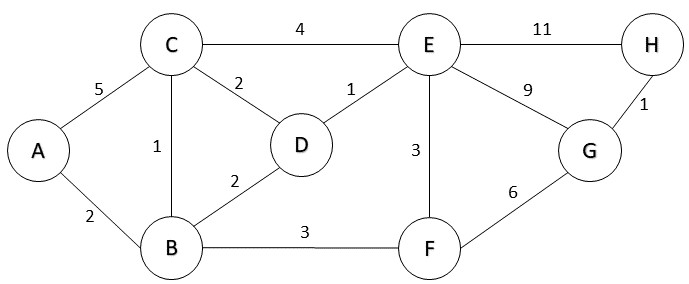
\includegraphics[width=120mm]{undirected_graph2.png}
	\caption{Ένα μη κατευθυνόμενο γράφημα 8 κορυφών με βάρη στις ακμές του}
	\label{fig:undirected_graph2}
\end{figure}

Ο ακόλουθος πίνακας δείχνει την εκτέλεση του αλγορίθμου
\begin{table}[ht!]
	\centering
	\label{tbl:dijkstra3}
	\begin{tabular}{|c|c|c|c|c|c|c|c|c|}
		\hline
		Σύνολο $S$            & A & B        & C        & D        & E        & F        & G        & H         \\ \hline
		$\{\}$                & 0 & $\infty$ & $\infty$ & $\infty$ & $\infty$ & $\infty$ & $\infty$ & $\infty$  \\ \hline
		$\{A\}$               & 0 & $2_A$    & $5_A$    & $\infty$ & $\infty$ & $\infty$ & $\infty$ & $\infty$  \\ \hline
		$\{A,B\}$             & 0 & $2_A$    & $3_B$    & $4_B$ & $\infty$ & $5_B$    & $\infty$ & $\infty$  \\ \hline
		$\{A,B,C\}$           & 0 & $2_A$    & $3_B$    & $4_B$    & $7_C$    & $5_B$    & $\infty$ & $\infty$  \\ \hline
		$\{A,B,C,D\}$         & 0 & $2_A$    & $3_B$    & $4_B$    & $5_D$    & $5_B$    & $\infty$ & $\infty$  \\ \hline
		$\{A,B,C,D,E\}$       & 0 & $2_A$    & $3_B$    & $4_B$    & $5_D$    & $5_B$    & $14_E$   & $16_E$    \\ \hline			
		$\{A,B,C,D,E,F\}$     & 0 & $2_A$    & $3_B$    & $4_B$    & $5_D$    & $5_B$    & $11_F$   & $16_E$    \\ \hline			
		$\{A,B,C,D,E,F,G\}$    & 0 & $2_A$    & $3_B$    & $4_B$    & $5_D$    & $5_B$    & $11_F$   & $12_G$    \\ \hline			
		$\{A,B,C,D,E,F,G,H\}$ & 0 & $2_A$    & $3_B$    & $4_B$    & $5_D$    & $5_B$    & $11_F$   & $12_G$    \\ \hline
	\end{tabular}
	\caption{Συνοπτική εκτέλεση του αλγορίθμου}
\end{table}


Οι συντομότερες διαδρομές είναι:
\begin{itemize}[noitemsep]
\item Για την κορυφή A η διαδρομή είναι η A με μήκος 0
\item Για την κορυφή B η διαδρομή είναι η A-B με μήκος 2
\item Για την κορυφή C η διαδρομή είναι η A-B-C με μήκος 3
\item Για την κορυφή D η διαδρομή είναι η A-B-D με μήκος 4
\item Για την κορυφή E η διαδρομή είναι η A-B-D-E με μήκος 5
\item Για την κορυφή F η διαδρομή είναι η A-B-F με μήκος 5
\item Για την κορυφή G η διαδρομή είναι η A-B-F-G με μήκος 11
\item Για την κορυφή H η διαδρομή είναι η A-B-F-G-H με μήκος 12
\end{itemize}

\subsection{Παράδειγμα 2}
Γράψτε πρόγραμμα που να διαβάζει ένα γράφημα και να εμφανίζει για κάθε κορυφή το βαθμό της, δηλαδή το πλήθος των κορυφών με τις οποίες συνδέεται απευθείας καθώς και το μέσο όρο βαρών για αυτές τις ακμές. Επιπλέον για κάθε κορυφή να εμφανίζει τις υπόλοιπες κορυφές οι οποίες μπορούν να προσεγγιστούν με διαδρομές μήκους 1,2,3 κοκ.

\lstinputlisting[caption = (lab08\_ex2.cpp),multicols=2]{lab08/lab08_ex2.cpp}

Η μεταγλώττιση και η εκτέλεση του κώδικα γίνεται με τις ακόλουθες εντολές:

\lstinputlisting[style=DOS]{lab08/compile_execute3.txt}

Η δε έξοδος που παράγεται είναι η ακόλουθη:

\lstinputlisting[style=DOS]{lab08/lab08_ex2.out}

\section{Ασκήσεις}
\begin{enumerate}[nolistsep]
	\item Υλοποιήστε τον αλγόριθμο των Bellman-Ford \cite{brilliant_bellman_ford} για την εύρεση της συντομότερης διαδρομής από μια κορυφή προς όλες τις άλλες κορυφές.
	\item Υλοποιήστε έναν αλγόριθμο τοπολογικής ταξινόμησης για DAGs \cite{g4g_topological_sort}.
\end{enumerate}

\begin{thebibliography}{9}
\bibitem{g4g_graph_representations}
Geeks for Geeks, graphs and its representations, \href{https://www.geeksforgeeks.org/graph-and-its-representations/}{https://www.geeksforgeeks.org/graph-and-its-representations/}

\bibitem{he_graph_representations}
HackerEarth, graph representation, \href{https://www.hackerearth.com/practice/algorithms/graphs/graph-representation/tutorial/}{https://www.hackerearth.com/practice/algorithms/graphs/graph-representation/tutorial/}

\bibitem{pa_floyd_warshall}
Programming-Algorithms.net, Floyd-Warshall algorithm, \href{http://www.programming-algorithms.net/article/45708/Floyd-Warshall-algorithm}{http://www.programming-algorithms.net/article/45708/Floyd-Warshall-algorithm}

\bibitem{programiz_prim}
PROGRAMIZ, Prim's algorithm, \href{https://www.programiz.com/dsa/prim-algorithm}{https://www.programiz.com/dsa/prim-algorithm}

\bibitem{programiz_kruskal}
PROGRAMIZ, Kruskal's algorithm, \href{https://www.programiz.com/dsa/kruskal-algorithm}{https://www.programiz.com/dsa/kruskal-algorithm}

\bibitem{g4g_topological_sort}
Geeks for Geeks, topological sorting, \href{https://www.geeksforgeeks.org/topological-sorting/}{https://www.geeksforgeeks.org/topological-sorting/}

\bibitem{dicretetext_euler_path}
Discrete Mathematics: An open introduction by Oscar Levin, Euler Paths and Circuits, \href{http://discretetext.oscarlevin.com/dmoi/sec_paths.html}{http://discretetext.oscarlevin.com/dmoi/sec\_paths.html}

\bibitem{he_scc}
HackerEarth, Strongly Connected Components, \href{https://www.hackerearth.com/practice/algorithms/graphs/strongly-connected-components/tutorial/}{https://www.hackerearth.com/practice/algorithms/graphs/strongly-connected-components/tutorial/}

\bibitem{brilliant_bellman_ford}
Brilliant.org, Bellman-Ford Algorithm, \href{https://brilliant.org/wiki/bellman-ford-algorithm/}{https://brilliant.org/wiki/bellman-ford-algorithm/}

\bibitem{algorithm_visualization_dijkstra}
Algorithm visualization, Dijkstra's shortest path, \href{https://www.cs.usfca.edu/~galles/visualization/Dijkstra.html}{https://www.cs.usfca.edu/~galles/visualization/Dijkstra.html}

\end{thebibliography}
